\documentclass[12pt, titlepage]{article}
\usepackage{longtable}
\usepackage{booktabs}
\usepackage{tabularx}
\usepackage{hyperref}
\hypersetup{
    colorlinks,
    citecolor=black,
    filecolor=black,
    linkcolor=red,
    urlcolor=blue
}
\usepackage[round]{natbib}
\usepackage{longtable}
\usepackage{graphicx}
\usepackage{enumerate}
\usepackage{amssymb}
\usepackage{amstext}
\usepackage{amsthm}
\usepackage{amsmath}
\usepackage{soul}
\usepackage{xcolor}

\title{SE 3XA3: Software Requirements Specification}

\author{Team 10, MacLunky
		\\ Albert Zhou, zhouj103
		\\Abeer Al-Yasiri, alyasira
		\\ Niyatha Rangarajan, rangaran
}

\date{\today}

\begin{document}

\maketitle

\pagenumbering{roman}
\tableofcontents
\listoftables
\listoffigures

\begin{table}[hp]
\caption{Revision History} \label{TblRevisionHistory}
\begin{tabularx}{\textwidth}{llX}
\toprule
\textbf{Date} & \textbf{Developer(s)} & \textbf{Change}\\
\midrule
February 9, 2021 & Albert, Abeer, Niyatha & Version 0 made\\
\hline
\textcolor{red}{March 30, 2021} & \textcolor{red}{Abeer}& \textcolor{red}{NFR}\\
\hline
\textcolor{red}{April 1, 2021} & \textcolor{red}{Albert} & \textcolor{red}{FR and Symbolic parameter and NFR}\\
\hline
\textcolor{red}{April 8, 2021} & \textcolor{red}{Albert} & \textcolor{red}{New requirements}\\
\bottomrule
\end{tabularx}
\end{table}

\newpage

\pagenumbering{arabic}

This document describes the requirements for MacLunky. The template for the Software Requirements Specification (SRS) is a subset of the Volere template~\citep{RobertsonAndRobertson2012}. If you make further modifications to the template, you should explicity state what modifications were made.

\section{Project Drivers}

\subsection{The Purpose of the Project}

The purpose of the project is developing a creative, interactive, and fully functional game version of Spelunky game using the Python2 open source version. The game is to be redeveloped in an innovative and more accessible way to be more appealing to the gaming community and to be easily accessed for any user who has access to the executable game. 

\subsection{The Stakeholders}

The stakeholders of the project include the gaming community which are the users of the product making them the primary stakeholders of the development course of the system. Also, the stakeholder includes all the interested parties of the system which are the clients, customers, and other associated parties interested in being secondary stakeholders. 

\subsubsection{The Client} 

The main clients of the project are the course instructor and the TAs as they are setting deadlines for project milestones and provide a view of customer feedback for project submissions. They are considered a primary stakeholder's because their requests and suggestions have the highest priority in the project development. In future advancements of the project, clients could include distribution platforms of the game. 

\subsubsection{The Customers}

The main customers of the product are the users. The users of the game will be desktop gamers of age 11 and above and demographic background who is interested in playing the game and has access to a PC. Another important customer base is interested developer parties such as the original game developers or the coding community interested in a learning opportunity and wants to see the project's merits and provide an outside opinion. 

\subsubsection{Other Stakeholders}

The secondary stakeholders who do not directly influence the project development are third parties interested in incorporating the project with their business goals. This could include advertising parties, open source platform users, industry experts, and McMaster University. Advertisers may request to show case business related artifacts to raise awareness for their brand while supporting the project's development. On the other hand, open source platforms are interested in showcasing the project to increase their project database choices. 
Industry experts could include anywhere from game companies interested in containing the game with their systems to game testers and technology experts. Also, McMaster University could be a secondary stakeholder as the project is being developed by a team of engineering students and they do represent the engineering faculty with the work the development team produces. 

\subsection{Mandated Constraints}

The project is constrained by the following:
\begin{enumerate}
    \item Project must be fully developed and completed by the preset deadline of April 12, 2021.
    \item Project must be developed incrementally and meets all the intermediate deliverables' deadlines as stated and outlined by the course instructor. 
    \item The project must redevelop an open source product and provide licensing of usage. 
    \item The runtime and quality of the game will be constrained by the user's computer software and monitor.
    \item The project is to be developed with 0\$ budget and using only free software resources.
    \item The product will be tested to be compatible with Windows OS. 
    \item The product must adhere to University and course instructor's guidelines. 
    \item Due to limited time and resources, the project will prioritize meeting project requirements over graphic design. 
    \item The graphics functionality of the game will be limited by Pygame library resources. 
\end{enumerate}

\subsection{Naming Conventions and Terminology}

The sections will provide this document's terminology definitions and a list of the project's naming conventions and vocabulary. 
\begin{itemize}
    \item OS: Operating system. 
    \item Python: An OOP language used in the project development. The older version is Python2 and the most recent version Python3.
    \item Pygame: Computer graphics Python library. The most common game development Python library.
    \item Pylunky: The open source original Python Spelunky game being used for the project. 
    \item Spelunky: The original fully functional released game that provides a reference point for the new game objective. 
    \item MacLunky: The new redevelopment game in Python3 for this project. 
    \item Interface: The main game graphics and user application created by Pygame library. 
    \item User: The player who will be directly interacting with the game. This is one of the project's primary stakeholders. 
    \item Help Display: The game's help functionality includes instructions on how to interact with the game.
    \item Map: A file containing the entire layout of a level including blocks, enemies, traps, chests, signs, and doors.
    \item Level: A 2D area the user explores.
    \item Camera: The view of a level.
    \item Heart: Represents the user's health points in the game. 
    \item Screen: The game window interface where the game map and features are displayed. 
\end{itemize}

\subsection{Relevant Facts and Assumptions}

The relevant project facts include information on the original project code, design and technology. This includes the following:
\begin{itemize}
    \item The original game open source Pylunky is implemented using Python2 and deployed using Pygame. 
    \item The original game graphics and features is limited by the available resources of Pygame to create the game from the Python files. 
    \item The original project implementations had 646 lines of code.
    \item The original game was released as a zip file to be played by running a main game python file.
\end{itemize}
The project assumptions are related to defining user characteristics and how the game is expected to interact with the environment. Assumptions will include any decisions that directly affect the project development. The assumptions include the following:
\begin{itemize}
    \item The project will be able to use the original game open source files to build on and reshape the new game's features. 
    \item The project will be able to meet all the game's graphic requirements using Pygame library.
    \item The project will aim to recreate a different instance of the game to increase the game's excitement level. 
    \item The project assumes that the user has access to Pygame and Python to run the game files. 
    \item The project assumes the user knows how to run and play a desktop game using zip file released format. 
    \item The project assumes the user will be able to follow the game's instructions and understand the different symbols on the game screen. 
\end{itemize}

\section{Functional Requirements}

\subsection{The Scope of the Work and the Product} %Abeer

The project will undertake the redevelopment of the Spelunky Python game version to add advanced new game features and implement a creative approach of how the player will interact with the system. The scope of the project will include a new Python3 implementation of the game with a running executable file as a user's interface and to introduce detailed documentation of the system's software and design. The new product will be released under the name "MacLunky". MacLunky is a single-player game that takes place in a 2D maze mapping with entry and exit points. The game's objective is to reach the exit door by following a specific winning path in the maze and completing the challenges presented along the way. The goal of the project is to introduce new customized game maps and incorporate interactive challenges and objects along the path of the game. The final product should be an executable game with functional interactive game features. The new project additions will include customized game maps that introduce new challenges the player must overcome to meet the game's objective. The player will be able to explore the map by moving forward, backward, up, and down the paths of the map. Not only that the player will be able to interact with objects placed on the map by collecting treasures that reward the player with bonuses, by avoiding path obstacles, and by fighting enemies to progress in the game. The new product will produce a working interactive game functionality with new creative map exploration that gives the user a new engaging experience of, the redeveloped game, MacLunky. 

\subsubsection{The Context of the Work} 

The original Pylunky has poor implementation documentation and not a fully functional game platform for the user to interact with to win the game. The original open source game files act as Spelunky Python version "tech demo" to illustrate a snapshot of the game design outline and starting point. Not only does Pylunky fail to deliver a user friendly game but it also fails to meet the software engineering design principle and process. Pylunky is not ideal for a developer to understand the game's file structure and working software as it lacks documentation and modular design in the project. Therefore, MacLunky has two goals: one, to redesign the game following software engineering principles and process for the benefit of other developers, and two, to give the user an interactive and engaging game with an understandable winning criteria and functionality.  

\subsubsection{Work Partitioning}

\begin{longtable}{|p{0.2\linewidth}|p{0.25\linewidth}|p{0.26\linewidth}|p{0.3\linewidth}|}
    \caption{Work Partitioning}
    \\
    \hline
	Event Name & Input & Output & Summary\\
	\hline
    Start Game & Developer graphics and code & Pygame, executable window & Creates the game's maze level with the multiple paths starting from the player's entry position to the game's exiting point. Produces the game's outline to be presented to the user on the screen. It includes 3 different map designs to create the game from.\\
	%\hline
	%Game Objects & Developer graphics and code & Pygame, executable window & Creates and positions the game's objects on the game level.\\
	\hline
	Fight Enemy & Keyboard inputs & Pygame, display enemy character & Based on the user action inputs the player's character will attack the enemy that is controlled by the system.\\
	\hline
	Open Treasure & Keyboard inputs & Pygame, display object and save it to the user's resources & The user will open the treasure box that was placed by the system on the game's path.\\
	\hline
	Exit Game & Keyboard input & Exit game window & Upon the player reaching the end of the path to have met the winning criteria of the game the game will shut down and close the game window.\\
	\hline
	Access Help & keyboard/mouse input & Pygame, message note & Upon the user passing by an object or moving the cursor to view the help message of the game that includes the game's user instructions and guidelines.\\
	%\hline
	%Game Generation & Developer code & Pygame, executable window & Creates the game window and places all the interactive and user related features on it. It randomly selects one game mapping design to be presented for user this game instance.\\
	%\hline
	%Game Timer & Developer code & Pygame, executable window & Creates and starts the timer of the game. It will be displayed on the game screen for the user to see and to be saved later upon winning the game.\\
	\hline 
	Character Moves & Keyboard input & Pygame, character changes position & Different keyboard input will represent the character moving up, down, left, right, jump, hit, throw, and climb. It will include the allowed user actions in an interactable game mode to progress in the game and meet the winning criteria of the game.\\
	\hline
	Game Over & keyboard input & Pygame, exit game window & Upon the player losing all life points, hearts, the system will shut down and exits the window.\\
	\hline
	Collects Bomb & Keyboard input & Pygame, stores the bomb in the user's resources & Upon user collecting the bomb while moving around in the game. This acts as a defense strategy of the player to defeat approaching enemies. \\
	\hline
	Throw Bomb & Keyboard input & Pygame, Bomb explodes & Upon the user action to throw the bomb an explosion will happen destroying what is infront of the user character on the path This could be fighting method against enemies or to clear the path by destroying blocks.\\
	\hline
	%Climb Rope & Keyboard input & Pygame, execut & Upon the creation of a rope, it is thrown up from the player or placed at their feet. With the rope, the player is able to advance up and down map locations to ultimately dodge enemies or approach the level exit sooner.\\
	%\hline
\end{longtable}

\newpage

\subsubsection{Individual Product Use Cases}

\begin{figure}[h!]
    \centering
    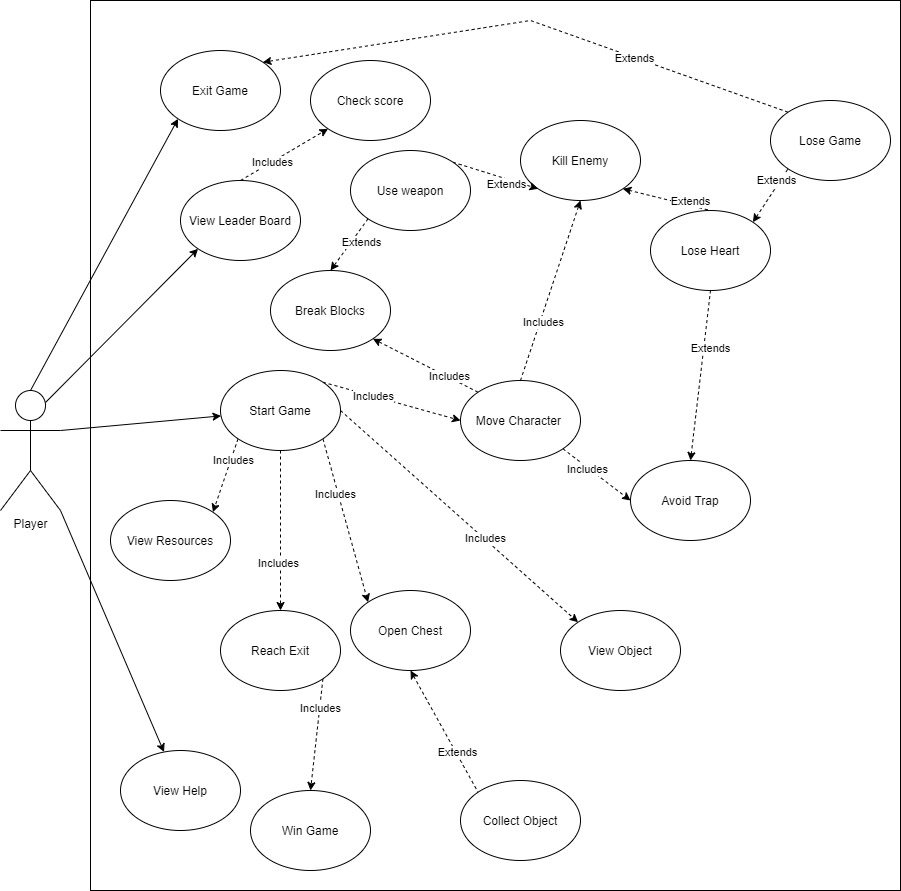
\includegraphics[scale=0.5]{xa3_usecase.jpg}
    \caption{Use Case Diagram}
\end{figure}

\newpage

\begin{longtable}{|l|p{0.75\linewidth}|}
\caption{Use Case Description}\\
\hline
Use Case & Description\\
\hline
Exit Game & The user wants to quit the game by exiting the game window application.\\
\hline
View Leader Board & The user wants to access the top scores of the game where the system stores all the previous game score in descending order. The user's score is a culmination of both play time and treasure objects collecting during the course of game play.\\
\hline
Check Score & The user searches for their specific score in the leader board system of the game. \\
\hline
View Help & The user views the rules of the game through signs throughout the level or through the user guide.\\
\hline
Start Game & The user starts the game. The system creates a level from a map design, populates it with enemies, chests, traps, doors. and signs and place the player at the entrance door.\\
\hline
View Resources & The user views their hearts, bombs, ropes, gold, and time.\\
\hline
Reach Exit & The user goal is to find the exit point of the game to win the game by exploring the level. The exit is reached at the end of the path of the game.\\
\hline
Win Game & The user wins the game by reaching the exit point in the game which is represented by a door. The user is prompted to save their score and their name. The top scores are then displayed.\\
\hline
Open Chest & The user interacts with a chest sending an assortment of objects out. The user is able to increase their defense strategy through weapon objects or increase their score through treasure objects.\\
\hline
Collect Object & The user collects objects by touching them when they move over the object. Collected treasure is added to the user's gold amount and resources.\\
\hline
View Object & The user reads the message of an object when passing by it. The message is displayed at the bottom of the screen. This gives the user an idea of what milestone they have achieved at that point in the game.\\
\hline
Move Character & The user wants to control the character to move up, down, left, right, climb, attack, and jump.\\
\hline
Break Blocks & The user places a bomb and destroys a solid block with the explosion, turning it to an empty block. This helps the user dodge approaching enemies faster and can even allow them to progress closer to the level exit faster.\\
\hline
Avoid Trap & The users dodges an arrow or avoids landing on a spike by moving the character to a safe position or using special character actions.\\
\hline
Use Weapon & The user want to carry a weapon and use it to defend themselves against enemies or clear the path of the game.\\
\hline
Kill Enemy & The user kills an enemy with a bomb, weapon, trap, or by stomping on them. As a result the enemy will be destroyed if the user is successful in the attack.\\
\hline
Lose Heart & The user is attacked by an enemy or falls too far then takes loses a heart. This is an indicator of a user's health and hence the user must maintain a health of more than 0 hearts to stay in the game.\\
\hline
Lose Game & Upon the user losing all hearts the game terminates.\\
\hline
\end{longtable}

\subsection{Functional Requirements}

%numbering to be done once finalized
\textbf{Launch/Termination}\\
\textbf{FR1:} The system shall load a level when launched.\\
\textbf{FR2:} The system shall be able to be closed at any time with keyEsc.\\ 
\\
\textbf{Display}\\
\textbf{FR3:} The screen shall display everything in view of the camera.\\
\textbf{FR4:} The camera shall follow the player and stay within the boundaries of the level.\\
\textbf{FR5:} The player's hearts, bombs, ropes, gold, and time shall always be displayed in the top left corner of the screen, over the camera.\\
\\
\textbf{Player}\\
\textbf{FR6:} The player shall be able to move the camera up with keyUp or down with keyDown when standing.\\
\textbf{FR7:} The player shall be able to move left with keyLeft, move right with keyRight, and jump with keyJump.\\
\textbf{FR8:} The player shall be able to interact with chests and doors with keyInt.\\
\textbf{FR9:} The player shall be able to place a bomb at their feet with keyBomb.\\
\textbf{FR10:} The player shall be able to throw a rope up with keyRope.\\
\textbf{FR11:} The player shall be able to place a rope at their feet with keyDown and keyRope.\\
\textbf{FR12:} The player shall be able to use their with keyweap.\\
\textbf{FR13:} The player shall start the level with heartStartAmount hearts, bombStartAmount bombs, and ropeStartAmount ropes.\\
\textbf{FR14:} The player shall move at a speed of playerSpeed \st{blocks} \textcolor{red}{pixels} per second.\\
\textbf{FR15:} The player shall jump to a height of playerJumpHeight tiles in playerJumpSpeed seconds.\\
\\
\textbf{Bomb}\\
\textbf{FR16:} A bomb shall explode after bombTime seconds and destroy all blocks, enemies, traps, signs, and the player in a bombSize block explosion.\\
\textbf{FR17:} A bomb at the player's feet shall be picked up by the player with keyDown and keyweap.\\
\textbf{FR18:} A bomb shall be thrown forward by keyweap at throwSpeed \st{blocks} \textcolor{red}{pixel} per second.\\
\textbf{FR19:} A thrown bomb shall explode immediately when colliding with \st{any object} \textcolor{red}{a solid block}.\\
\\
\textbf{Rope}\\
\textbf{FR20:} A rope shall be thrown up to Ropelength blocks high and attach to the bottom of a block.\\
\textbf{FR21:} A rope shall extend Ropelength blocks down.\\
\textbf{FR22:} The player shall grab the rope with keyUp when near it.\\
\textbf{FR23:} The player must be able to move along the rope up with keyUp or down with keyDown.\\
\textbf{FR24:} The player shall release the rope with keyJump.\\
\\
\textbf{Weapon}\\
\textbf{FR25:} The player shall be able to use their weapon in an area in front of them.\\
\textbf{FR26:} An enemy hit by the weapon shall take weaponDmg damage.\\
\textbf{FR27:} The player shall be able to use the weapon once every weaponDelay seconds.\\
\\
\textbf{Movement}\\
\textbf{FR28:} The player shall not be able to move through solid tiles or past the level boundaries.\\
\textbf{FR29:} The player shall be able to lose hearts from falling too fast or being hit by an enemy.\\
\textbf{FR30:} The player shall lose fallDmg hearts after falling over fallDmgDist blocks.\\
\\
\textbf{Gold}\\
\textbf{FR31:} The gold shall be the sum of all treasure the player has collected.\\
\textbf{FR32:} The player shall collect treasure when \st{touching} \textcolor{red}{using} it.\\
\st{\textbf{FR33:} The system shall start a timer from instance the player was placed at the entrance point.}\\
\\
\textbf{Sprite}\\
\textbf{FR34:} The player's sprites shall reflect their movement.\\
\\
\textbf{Enemy Behaviour}\\
\textbf{FR35:} An enemy shall be able to move around the level.\\
\textbf{FR36:} An enemy shall be able to hit the player.\\
\textbf{FR37:} If the player jumps on an enemy, the player shall bounce off and deal stompDmg to them.\\
\textbf{FR38:} If an enemy hits the player, the player shall be immune to damage for a short time.\\
\\
\textbf{Chest}\\
\textbf{FR39:} The system shall be able to place chests in a level.\\
\textbf{FR40:} The player shall be able to open chests with keyInt.\\
\textbf{FR41:} A chest shall contain a selection of treasure or bombs or ropes.\\
\textbf{FR42:} The contents of a chest shall fly out when opened and are collected by the player when touching them.\\
\textbf{FR43:} Treasure shall refer to diamonds, rubies, sapphires, emeralds, and gold bars.\\
\textbf{FR44:} A diamonds shall be worth valDiamond gold.\\
\textbf{FR45:} A ruby shall be worth valRuby gold.\\
\textbf{FR46:} A sapphire shall be worth valSapphire gold.\\
\textbf{FR47:} An emerald shall be worth valEmerald gold.\\
\textbf{FR48:} A gold bar shall be worth valGoldBar gold.\\
\\
\textbf{Enemy Types}\\
\textbf{FR49:} Enemies shall include snakes and spiders.\\
\\
\textbf{Snake}\\
\textbf{FR50:} A snake shall move left or right.\\
\textbf{FR51:} A snake shall change direction if the block in front of them is solid or if they would fall off the edge of a solid block.\\
\textbf{FR52:} A snake shall move at snakeSpeed tiles per second.\\
\textbf{FR53:} A snake shall have snakeHearts hearts.\\
\textbf{FR54:} A snake shall deal snakeDmg damage to the player.
\\
\textbf{Spider}\\
\textbf{FR55:} A spider shall be dormant or active.\\
\textbf{FR56:} A spider must be active if the player is within spideSense tiles of it and dormant otherwise.\\
\textbf{FR57:} A spider shall not move if it is dormant.\\
\textbf{FR58:} A spider shall jump in the direction of the player if it is active.\\
\textbf{FR59:} A spider shall jump to a height of spideJumpHeight tiles and a distance of spideJumpDist tiles in spiderJumpTime seconds.\\
\textbf{FR60:} A spider shall jump every spiderJumpDelay seconds.\\
\textbf{FR61:} A spider shall have spiderHearts hearts.\\
\textbf{FR62:} A spider shall deal spiderDmg damage to the player.\\
\\
\textbf{Trap Types}\\
\textbf{FR63:} Traps shall include arrow traps and spikes.\\
\\
\textbf{Arrow Trap}\\
\textbf{FR64:} An arrow trap shall be placed on top or on the side of a solid block.\\
\textbf{FR65:} An arrow trap shall face either left or right.\\
\textbf{FR66:} An arrow trap shall fire an arrow in the direction it is facing if there is any movement within arrowSense blocks in front of it.\\
\textbf{FR67:} An arrow trap shall fire only arrowNum arrows.\\
\textbf{FR68:} An arrow trap shall fire an arrow with a speed of arrowSpeed tiles per second.\\
\textbf{FR69:} An arrow shall not be affected by gravity while flying.\\
\textbf{FR70:} An arrow shall stop and fall to the ground if it hits an enemy, the player, or a solid block.\\
\textbf{FR71:} An arrow shall deal arrowDmg damage to the player or an enemy.\\
\\
\textbf{Spike}\\
\textbf{FR:72} A spike shall be placed on the top of a solid block.\\
\textbf{FR:73} A spike shall deal spikeDmg to the player or an enemy if it falls on to it.\\
\\
\textbf{Game Ending}\\
%The game shall load another level when the player reaches the current level's exit.\\
%\textbf{FR:} If the player loses all of their hearts, the game shall give the player the option to restart the game with keyJump.\\
\textcolor{red}{\textbf{FR74:} If the player loses all of their hearts, the game must terminate.}\\
\textbf{FR75:} If the player interacts with the exit door, the game shall save their score \st{and prompts the user to enter a nameLength letter name and then display the leader board}.\\
\textbf{FR76:} The score shall be determined by scoreCalc.\\
\textbf{FR77:} The top score shall be displayed \textcolor{red}{and saved on score record file} \st{with keyScoreboard}.\\
\\
\textbf{Level}\\
\textbf{FR78:} The game shall create a level based on a map.\\
\textbf{FR79:} A map shall contain the entire layout of the blocks of the level, the locations of the entrance and exit doors, and all signs, chests, chest contents, enemies, and traps.\\
\textbf{FR80:} The player shall start the level at the entrance door.\\
\textbf{FR81:} The map shall contain at least one path of empty blocks from the entrance to the exit.\\
\textbf{FR82:} Blocks shall be solid or empty.\\
\textbf{FR83:} Solid blocks shall be impassable to the player and enemies, and can have traps or signs attached to them.\\
\textbf{FR84:} Empty blocks shall be passable to the player and enemies, and can not have traps or signs attached to them.\\
\\
\textbf{Sign}\\
\textbf{FR85:} The game shall use signs to communicate the rules to the player.\\
\textbf{FR86:} A sign shall display a message.\\
\textbf{FR87:} Sign messages shall be displayed at the bottom of the screen such that they are readable regardless of the background tiles.\\ 
\\
\textbf{Other}\\
\textcolor{red}{\textbf{FR88:} A bomb pile shall contain valBombPile bombs.}\\
\textcolor{red}{\textbf{FR89:} A rope pile shall contain valRopePile ropes.}\\
\textcolor{red}{\textbf{FR90:} Arrows shall be picked up and thrown at throwSpeed by the player.}\\
\textcolor{red}{\textbf{FR91:} Chests shall be picked up and thrown at throwSpeed by the player.}\\


Fit criteria: The behaviour of all modules shall be observed and measured to verify that they meet the functional requirements.

\section{Non-functional Requirements}

\subsection{Look and Feel Requirements}
\textbf{NFR1:} The game shall give a feel similar to that of Spelunky Classic.\\
%Fit Criteria Rationale: The users shall interact with game settings that are adopted from the original game colour scheme and background settings.  \\\\ 
Fit Criteria Rationale: At least 80\% surveyed users who have played Spelunky Classic agree that MacLunky gives a similar look and feel.\\\\
%\textbf{NFR2:} The game must involve interaction with the level and entities present on said level.\\ %NFR? how does it relate to look and feel? the user must feel like they are the one interacting with things and not just playing a game (immersion)- criteria: survey on player's feelings
%Fit Criteria Rationale: The game must contain doors to move in and out of doors present on the level, collect treasure and even avoid enemies.\\\\
\textbf{NFR2:} The user shall feel like they are the one exploring the level and not just playing a game.\\
Fit Criteria Rationale: At least 80\% of surveyed users agree that MacLunky feels immersive.\\\\
\textbf{NFR3:} The user shall feel like they are the character.\\
Fit Criteria Rationale: The user's keystrokes must move an on-screen character's movement immediately after control initiation.\\
%Fit Criteria Rationale: The user's keystrokes and mouse controls must move an on-screen character's movement immediately after control initiation.\\
%\textbf{NFR3:} The player must have control over a character that explores the level.\\ %NFR? same as above. could say player feels like they are the character - criteria: survey on precise movement
%Fit Criteria Rationale: The user's keystrokes and mouse controls must move an on-screen character's movement immediately after control initiation.\\

\subsection{Usability and Humanity Requirements}

%\textbf{NFR4:} The game must have help and exit features available through game play\\ %NFR? the rules of the game should be self evident - criteria: ask users if they understood by playing or needed help from someone
%Fit Criteria Rationale: The game must have control/feauture-aid textboxes that answer user questions through the duration of gameplay.\\\\
\textbf{NFR4:} The rules of the game shall be apparent.\\
Fit Criteria Rationale: At least 80\% of recorded users should not require outside help.\\\\
\textbf{NFR5:} The game shall have easy-to-understand controls and game functionalities suitable for all audiences.\\
Fit Criteria Rationale: The game must be understandable to players of age 11 and above. The game must have suitable graphics in terms of content like violence and language with respect to the audience age.\\\\
\textbf{NFR6:} The user's progress in the level shall be apparent.\\
Fit Criteria Rationale: The game must contain signs detailing milestones in the level.\\\\
%\textbf{NFR6:} The game must have signs that aid in understanding which milestone say a level, they have reached in the map.\\
%Fit Criteria Rationale: The game must contain signs with legible font that help the user understand with point in the game they have reached. The signs must stay present for the duration of the game once it is reached by the player in the game.\\\\
\textbf{NFR7:} All user help and in game texts shall be legible for the user and its font style must be visually appealing.\\
Fit Criteria Rationale: The size of the font in the game must be legible and must follow the standard of \textcolor{red}{at least} 10 point size \st{Verdana}.\\

%plays like spelunky classic, suitable for all audiences

\subsection{Performance Requirements}

\textbf{NFR8:} The system shall be able to respond to user input controls within 10ms of its initiation.\\
Fit Criteria Rationale: The response time of 10ms must be maintained for all game user-system interactions like mouse controls and keyboard/keypad strokes for at least 90\% of use time and be at most 15ms for the remaining tiem.\\\\
\textbf{NFR9:} The character controlled by the player shall have precise movements along the level with respect to other static or moving level entities.\\
Fit Criteria Rationale: The user must move such that the expected coordinates of a character's position in the level and any other entity (say an enemy) must not have any positional error. The coordinates of the character must be calculated as per the corner points of their 2-d block of space occupied on the grid.\\\\
\textbf{NFR10:} The game system shall have a stable framerate of at least \st{30} \textcolor{red}{90} fps.\\
Fit Criteria Rationale:The framerate must be kept at least \st{30} \textcolor{red}{90}fps for the duration of game play. \\\\
\textbf{NFR11:} The storage capacity required to download this game must be set to a relatively low value.\\
Fit Criteria Rationale: The user shall have a recommended 16GB to maintain good gaming performance without storage limitations and movement lags.\\
\textcolor{red}{\textbf{NFR25:} The game shall terminate with an error if necessary.\\
Fit Criteria Rationale: The system shall be tested for errors.\\}

\subsection{Operational and Environmental Requirements}

\textbf{NFR12:} The game shall have an executable version of the game to avoid prerequisites to run the game.\\
Fit Criteria Rationale:The user must be able to use a packaged executable version of the game which requires no previously downloaded platform for its usage.\\\\
%\textbf{NFR13:} The game shall be provide download instructions for known incompatible OS.\\
%Fit Criteria Rationale: The game must have a working version compatible with Windows OS. For other OS since the downloading abilities and available system requirements may differ, there must be instructions on how to handle the game in such different OS. \\
%run on python vm

\subsection{Maintainability and Support Requirements}

\textbf{NFR13:} The game shall follow a modular structure for different game views and features.\\
Fit Criteria Rationale: The game must follow \st{an MVC style of} \textcolor{red}{the principles of separation of concerns} programming structure and \textcolor{red}{modularization}.\\\\
\textbf{NFR14:} The game shall be easy to change and modify due to the presence of modules. \\
Fit Criteria Rationale: The game must be released in new versions in the case of incompatibilities with a Windows OS update.\\\\
\textbf{NFR15:} The game shall be well documented with a log of commit history to trace back certain implementation steps.\\
Fit Criteria Rationale:The game must use an automatic documentation generator like doxygen to enable future readers to understand the program with ease. \\\\
\textbf{NFR16;} The game shall incorporate the support platforms of pygame and python.\\
Fit Criteria Rationale: The game must follow the set of standards and rules for running the game inclusive of its limitations, advantages and syntactical language \\
%no maintenance after course

\subsection{Security Requirements}
\textbf{NFR17:} The game shall maintain confidentiality of user information.\\
Fit Criteria Rationale: The game must store all user information in a protected format and must not allow access to such information by third parties.\\\\
\textbf{NFR18:} The game shall maintain the integrity of the file system it is downloaded into and not inject malicious software.\\
Fit Criteria Rationale: The game must be downloaded in a separate directory to prevent tampering of other files. The game must not access files which are not in its directory of download.\\\\
\textbf{NFR19:} The game shall make sure that private fields and entities of the game must be kept secure and not accessible to the general public.\\
Fit Criteria Rationale: All fields of a class must be declared private and those need to be accessed by other classes must facilitate this access through suitable getter functions.\\

\subsection{Cultural Requirements}
\textbf{NFR20:} The game shall not incorporate any racist or discriminatory language or symbols that might offend a certain community.\\
Fit Criteria Rationale: There must be an email provided in the game help section to contact for reporting offensive content. Such reports must be maintained at a number of zero. \\
\subsection{Legal Requirements}
\textbf{NFR21:} The game shall follow the community guidelines set by the pygame and python platform.\\
Fit Criteria Rationale: The game must follow the set of standards and rules for running the game inclusive of its limitations, advantages and syntactical language. The game must also maintain the security standards laid out for its usage. \\\\
\textbf{NFR22:} The game shall take inspiration only from those projects which are properly licensed and open source.\\
Fit Criteria Rationale: The game implementation and execution means must not cause reasons for copyright infringement. Hence, all work must be properly referenced and documented. The game must use only licensed and open source software in the case where outsourcing of program is required. \\

\subsection{Health and Safety Requirements}
\textbf{NFR23:} The game shall not include flashing graphics or disturbing imagery.
Fit Criteria Rationale: The game must not be harmful for those with epilepsy problems and should thus follow guidelines that cater to such audience.\\\\
\textbf{NFR24:} The colour scheme selected for the game shall be catered to allowing larger game time with minimal eye strain.\\
Fit Criteria Rationale: The game must maintain a minimal game time of 1-2 minutes to allow the user to play multiple rounds and take breaks to prevent a long play-time for one seating. \\
%This section is not in the original Volere template, but health and safety are
%issues that should be considered for every engineering project.

\section{Project Issues}

\subsection{Open Issues}
By using Pygame standards we limit the game's performance, speed and resolution because the game is built solely on this platform. Furthermore, we can not predict future system compatibility in the case of OS updates. The game keeps track of a scoring system. If we incorporated a leaderboard system, we can not predict that the current gaming software platforms will be compatible with a constantly updated player leaderboard system.

\subsection{Off-the-Shelf Solutions}

The source code of the original Spelunky is available. However, because it is written using GameMaker Studio, it is not as easy to understand as Python. Also, GameMaker Studio requires a license and the source code is written for an older version.

\subsection{New Problems}
N/A

\subsection{Tasks}
The main source for task definition and completion is defined in the course outline and Gantt chart. The Gantt chart incorporates the due dates and milestones as per the course outline and also has a detailed subset of tasks outlined for each milestone completion. Apart from this the Gantt chart also has a resources tab that maintains the specific tasks assigned to each group member. In addition to this, the Gantt chart also provides a visually appealing planner that lists out what tasks are due for that day in the calendar. 

\begin{center}
    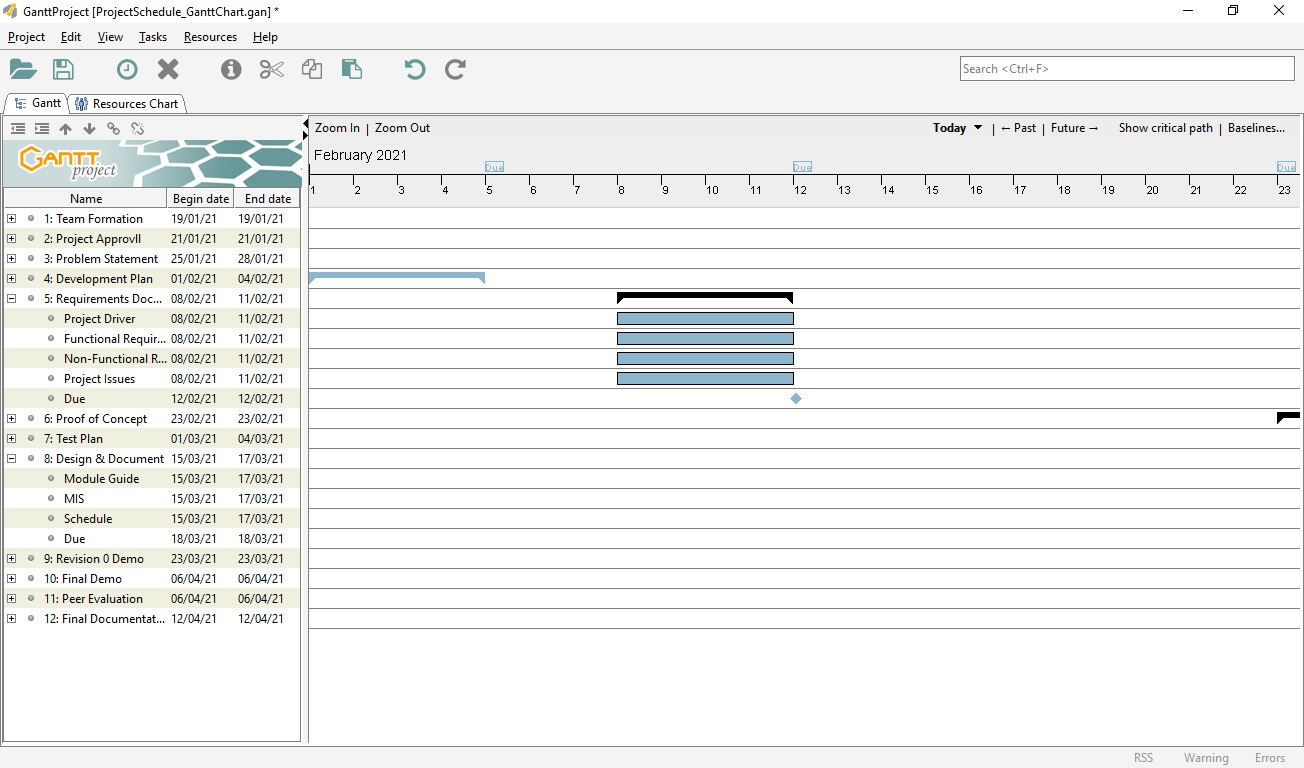
\includegraphics[scale=0.4]{Gantt1.jpg}
\end{center}

\subsection{Migration to the New Product}
N/A
\subsection{Risks}

The game is offline so there is no risk of unmonitored network access. The game collects no user data nor does it access files outside the game. There is no danger of physical harm to the user. Depending on the optimization, the game may cause the CPU to slowdown or overheat.

\subsection{Costs}

The project development and design should have no monetary costs as the team will be using open source libraries and tools. The development team will dedicate at least 2 hours of outside lab time for team meetings and 2 hours of individual work on the project weekly.

\subsection{User Documentation and Training}

The system will provide 3 means of user documentations and instructions:
\begin{enumerate}
    \item Instructions for the game will be presented to the user at the start of the game and the user will be able to access a HELP menu at any point in the game to understand the different game features and functionality.
    \item Installation document will be provided for the user to explain the procedure on how to download and prepare the user's OS environment to be able to play the game. 
    \item User manual will provide instructions and guidelines for how the game can be started using the released game version of the project and the basic functionality and rules of the game. The document will include an outline of the game features such as objects, the character, and enemies. Also, the document will contain a tutorial of the expected user-system interactions of starting the game and making a simple action in the game. This documentation will serve as the user training because the game is intuitive and has no learning curve to play the game.  
\end{enumerate}

\subsection{Waiting Room} 

In future project release, the game could take on further development on the graphics of the game to increase the game quality and user experience. The game could include sound effects to increase the user engagement with the game. Also, the system could increase it's users base by developing an app version of the game to make it accessible to non-desktop gamers. 

\subsection{Ideas for Solutions}

During the requirement planning stage, a few suggestions were made on implementation solutions. One possible solution is to use a one game screen to be the user interface that includes the game settings and the only user-system interaction point. Another, idea that was proposed is to use the exit point of the game as the winning criteria of the game. Hence, if the user completes the game's objective then the game shuts down and the system exits the application window. 

\bibliographystyle{plainnat}

\bibliography{SRS}

\newpage

\section{Appendix}

This section has been added to the Volere template.  This is where you can place
additional information.

\subsection{Symbolic Parameters}

The definition of the requirements will likely call for SYMBOLIC\_CONSTANTS.
Their values are defined in this section for easy maintenance.

\begin{longtable}{|l|p{0.5\linewidth}|p{0.25\linewidth}|}
\caption{Symbolic Parameter Table}\\
\hline
Symbolic Parameter & Description & Value\\
\hline
camWidth & The width of the camera, in pixels. & 320\\
\hline
camHeight & The height of the camera, in pixels. & 320\\

\hline
Symbolic Parameter & Description & Value\\
\hline
keyEsc & The key to quit the game. & esc key\\
\hline
keyLeft & The key to move left. & left arrow key\\
\hline
keyRight & The key to move right. & right arrow key\\
\hline
keyUp & The key to move/look up. & up arrow key\\
\hline
keyDown & The key to move/look down. & down arrow key\\
\hline
keyJump & The key to jump. & space key\\
\hline
keyInt & The key to interact. & tab key\\
\hline
keyBomb & The key to use a bomb. & b key\\
\hline
keyRope & The key to use a rope. & v key\\
\hline
% keyScoreboard & The key to display the scoreboard. & p key\\
% \hline
keyweap & The key to use the weapon. & left shift key\\
\hline
keyThrow & The key to throw object in empty space & left shift key\\
\hline
keyPick & The key to pick up object. & down arrow key and left shift key\\
\hline
keyCrouch & The key to crouch. & down arrow key\\
\hline


playerSpeed & The speed of the player in pixels per second. & 90\\
\hline
playerJumpHeight & The maximum height of the players jump in pixels. & 72\\
\hline
playerJumpSpeed & The speed the player reaches when jumping in pixels per second. & 3\\
\hline
playerClimbSpeed & The speed of the player in pixels per second when climbing. & 90\\
\hline

playerWidth & The width of the player, in pixels & 15\\
\hline
playerHeight & The height of the player, in pixels & 22\\
\hline

weaponDmg & The amount of damage dealt by the weapon. & 1\\
\hline
weaponDelay & The delay between weapon uses in seconds & 0.5\\
\hline
weaponAttack & The attack range of using the weapon in pixels & 16\\
\hline

fallDmg & The amount of damage the player takes when falling in blocks. & 1\\
\hline
fallDmgDist & The minimum fall distance in blocks the player must fall to take fall damage & 4\\
\hline

heartStartAmount & The number of hearts the player starts the level with. & 4\\
\hline
bombStartAmount & The number of bombs the player starts the level with. & 4\\
\hline
ropeStartAmount & The number of ropes the player starts the level with. & 4\\
\hline
bombTime & The number of seconds a bomb takes to explode. & 2\\
\hline
bombSize & The explosion size of a bomb in pixels. & 48.\\
\hline
throwSpeed & The speed of a thrown bomb in pixels per second. & 90\\
\hline

camWidth & The width of the camera, in pixels. & 320\\
\hline
camHeight & The height of the camera, in pixels. & 320\\

bombHeight & The width of a bomb, in pixels. & 12\\
\hline
bombWidth & The height of a bomb, in pixels. & 12\\
\hline
fallSpeed & The speed a bomb falls, in pixels per second. & 72\\
\hline
bombDmg & The amount of damage a bomb deals. & 10\\
\hline

Ropelength & The length of a rope in blocks. & 4\\
\hline

stompDmg & The amount of damage the player deals to an enemy when jumping on them. & 1\\
\hline

snakeSpeed & The speed of a snake in pixels per second. & 45\\
\hline
snakeHearts & The number of hearts a snake has. & 1\\
\hline
snakeDmg & The amount of damage dealt by a snake. & 1\\
\hline

spiderSense & The number of blocks to the player for a spider to be active. & 4\\
\hline
spideJumpHeight & The height a spider jumps in pixels. & 72\\
\hline
spideJumpDist & The distance a spider jumps in pixels. & 72\\
\hline
spiderJumpTime & The amount of time a spider is spent jumping in frames. & 24\\
\hline
spiderJumpDelay & The delay between spider jumps in seconds. & 2\\
\hline
spiderHearts & The number of hearts a spider has. & 1\\
\hline
spiderDmg & The amount of damage dealt by a spider. & 1\\
\hline

arrowSense & The number of blocks an arrow trap can detect movement. & 4\\
\hline
arrowNum & The number of arrows shot by an arrow trap. & 1\\
\hline
arrowSpeed & The speed of an arrow in pixels per second. & 90\\
\hline
arrowDmg & he amount of damage dealt by an arrow. & 2\\
\hline
spikeDmg & The amount of damage dealt by landing on a spike. & 4\\
\hline


valDiamond & The gold value of a diamond. & 5000\\
\hline
valRuby & The gold value of a ruby & 1600\\
\hline
valSapphire & The gold value of a sapphire. & 1200\\
\hline
valEmerald & The gold value of an emerald. & 800\\
\hline
valGoldBar & The gold value of a gold bar. & 500\\
\hline
\textcolor{red}{valBombPile} & \textcolor{red}{The number of bombs in a bomb pile.} & \textcolor{red}{3}\\
\hline
\textcolor{red}{valRopePile} & \textcolor{red}{The number of ropes in a rope pile.} & \textcolor{red}{3}\\
\hline
\st{nameLength} & \st{The number of characters of a name.} & \st{6}\\
\hline
scoreCalc & The score amount. & \st{\textbar gold - 100 * time(in seconds)\textbar} \textcolor{red}{the player's gold} \\
\hline
\end{longtable}


\end{document}
